
%% \textbf{@Pooyan,Andrea: here we should probably elaborate on OSTIA's architecture and the design principles that led us to define it as such... also we might want to elaborate on its components, the structure I'm suggesting below is merely tentative but it will give us ahead start!!}

%% \begin{itemize}
%% \item add and comment the meta-model of storm and how OSTIA uses that as a reference to draw and check models which are consistent with the technology
%% \item OSTIA Architecture
%% \item we should probably elaborate the architecture part (or on a separate "implementation" part or paragraph) with a link to the downloadable technology - @Andrea: can we bundle it up as plugin for Eclipse? E.g., somehow using RCP?
%% \item OSTIA Antipatterns Module
%% \item OSTIA Visualisation Module
%% \item OSTIA extensibility
%% \item OSTIA explanation of use and simple usage scenario
%% \item OSTIA explanation of use and simple usage scenario of continuous architecting
%% \end{itemize}
This section outlines OSTIA starting form a brief recap of the technology it is currently designed to support, i.e., the Apache Storm framework. Further on, the section introduces how OSTIA was designed to support continuous architecting of streaming topologies focusing on Storm. Finally, the section outlines the meta-model for Storm that captures all restrictions and rules (e.g., for configuration, topology, dependence, messaging, etc.) in the framework. OSTIA uses this meta-model as a reference every time the application is run to recover and analyse operational topologies.

\subsection{Storm architecture}

Storm is a technology developed at Twitter \cite{toshniwal2014storm} in order to
face the problem of processing of streaming of data. It is defined as a
distributed processing framework which is able to analyse streams of data. The
core element in the system is called \emph{topology}. A Storm topology is a
computational graph composed by nodes of two types: spouts and bolts. The former
type includes nodes that process the data entering the topology, for instance
querying APIs or retrieve information from a message broker, such as Apache
Kafka. The latter executes operations on data, such as filtering or serialising.

\subsection{OSTIA design}

The overall architecture of OSTIA is depicted in
Figure \ref{fig:ostia-arch}. The logical architectural information of the
topology is retrieved by OSTIA via static analysis of the source code. OSTIA
generates a simple intermediate format to be used by other algorithmic
processes.

OSTIA is architected in a way that algorithmic analysis, such as anti-pattern
analyses, can be easily added. These analyses use the information resides in the
intermediate format and provide added value analyses for continuous architecting
of storm topologies. Since the information in the intermediate format only rely
on the logical code analysis, some algorithmic analyses requires some
information regarding the running topology, such as end to end latency and
throughput.

Such information will be continuously added to the intermediate repository via
runtime monitoring of the topology on real deployment cluster. These provide
appropriate and rich information for refactoring the initial architecture and
enabling performance driven DevOps \cite{brunnert2015performance}.

Finally, OSTIA allows users to export the topology in different formats
(e.g. JSON) to analyse the topology with other tools.

\begin{figure*}[H]
	\begin{center}
		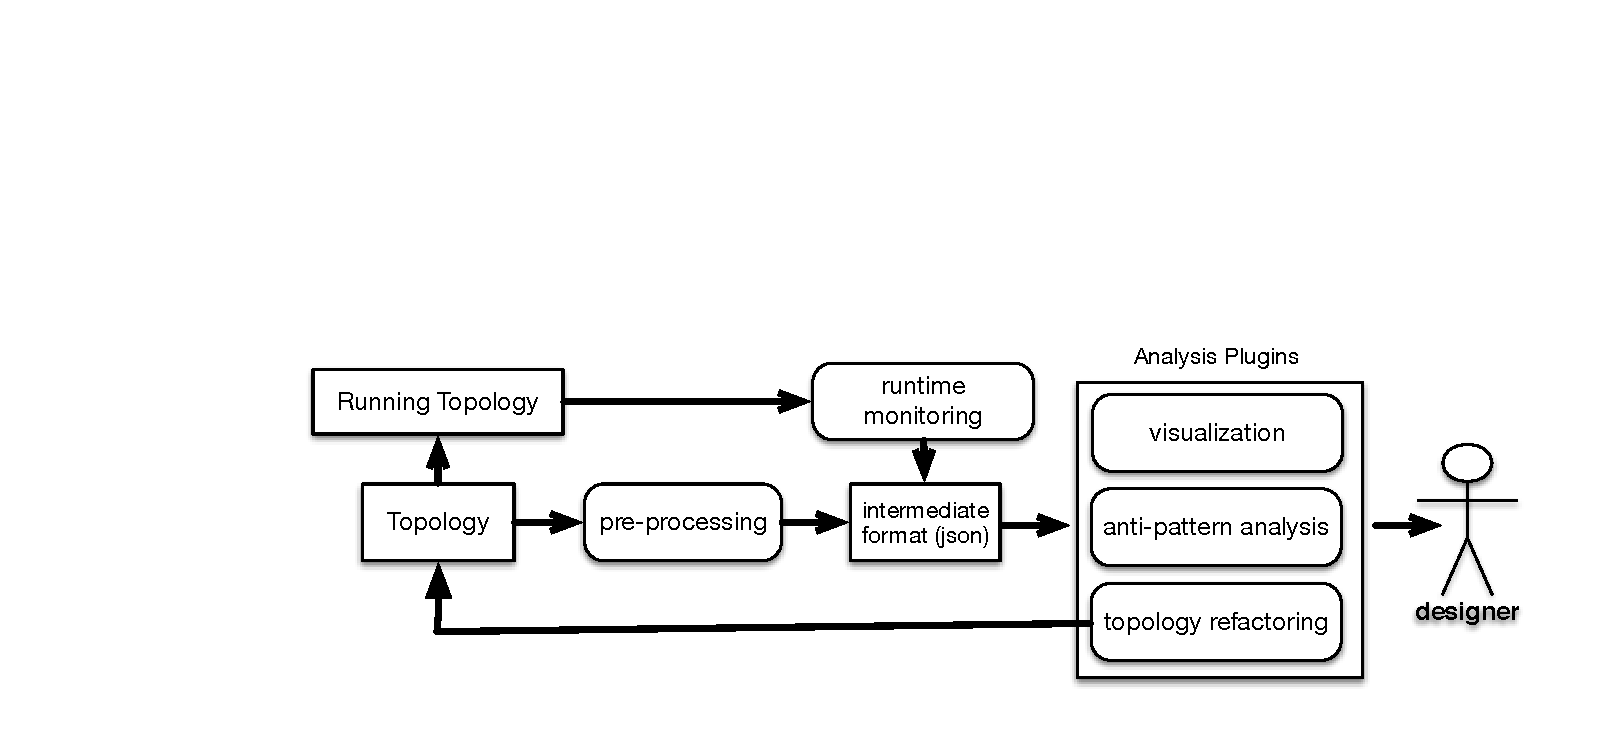
\includegraphics[width=8cm]{images/ostia-arch}
		\caption{OSTIA extensible architecture.}
		\label{fig:ostia-arch}
	\end{center}
\end{figure*}

\subsection{Deep Within OSTIA: The Storm Framework Meta-Model}

OSTIA was designed to retrieve and analyse Storm topologies on-the-fly, allowing their refactoring in a way which is consistent with framework restrictions, rules and regulations part of the Storm framework. In so doing, OSTIA uses a meta-model for the Storm framework. This meta-model acts as an image of all said restrictions and rules that OSTIA needs to maintain for elicited (or refactored) topologies. 
Essentially OSTIA implements in the meta-model the operational picture of the Storm Framework - this is critical to checking that the restrictions and constraints coded within Storm are reflected in elicited models as well as maintained during architecting and refactoring of those models. In addition, OSTIA applies all the necessary anti-pattern checks in combination with checking that said framework restrictions are maintained - this is critical to support continuous architecting in a manner which is consistent with Storm restrictions that would only become apparent during run-time and operations.
The meta-model in question is depicted in Fig. \ref{stormmm}. The figure shows an overview of the meta-model for Storm\footnote{The details of this meta-model and the restrictions captured therein is beyond the scope of this paper. More details are available in our project homepage, in section D2.1: \url{http://dice-h2020.eu/deliverables/D2.1}.} where, for example, the grouping restrictions that Storm envisions are captured in an enumeration of constraints (see the $<<$Grouping$>>$ element or the $<<$ReplicationFactor$>>$ concrete parameter). Key elements of the meta-model are the following:
\begin{itemize}
\item the $<<$TopologyConfiguration$>>$ meta-element contains the parameters necessary for the Storm framework to be configured and to run on the selected infrastructure. OSTIA checks that these parameters are present or that defaults are correctly inplace;
\item the $<<$TopologyConfiguration$>>$ meta-element specifies the topological construct being elicited for the analysed Storm application, as composed of the $<<$Bolt$>>$ and  the $<<$Spout$>>$ meta-elements;
\item  the $<<$Grouping$>>$ meta-element contains restrictions on the possible groupings of the $<<$Bolt$>>$ and the $<<$Spout$>>$ meta-elements within the elicited topology. OSTIA uses these restrictions to analyse the elicited topology;
\end{itemize}

\begin{figure*}
	\begin{center}
		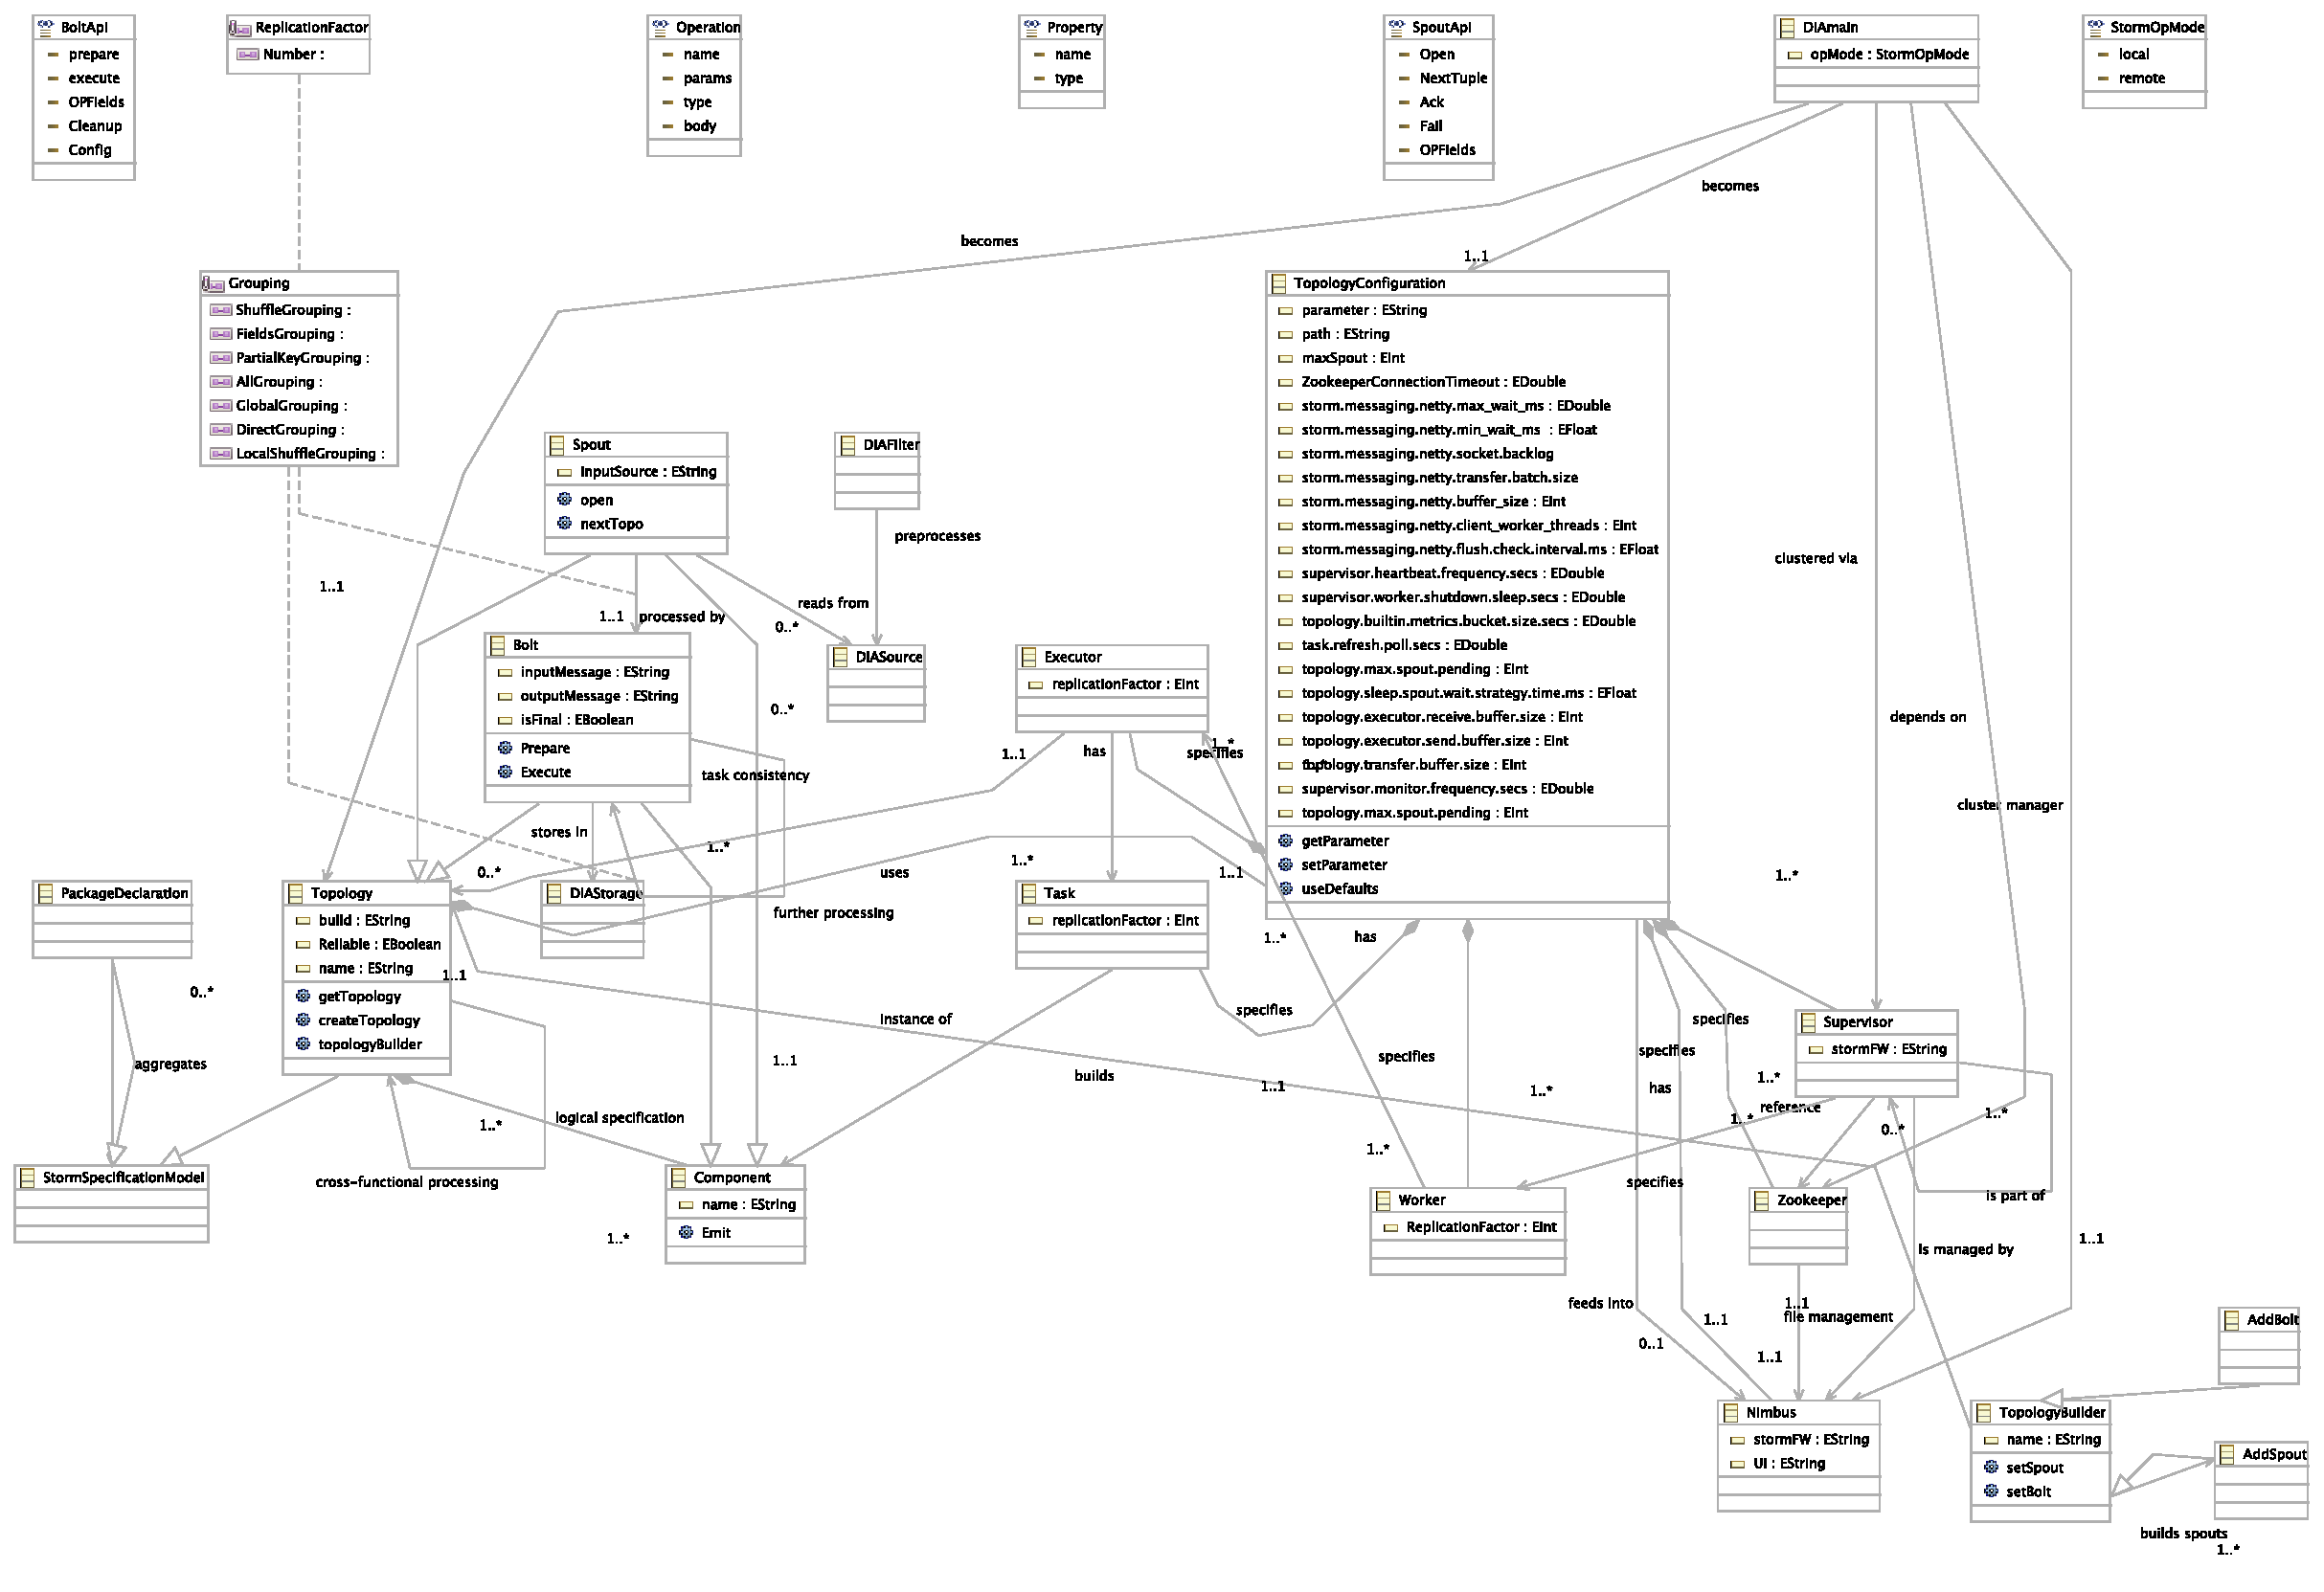
\includegraphics[width=18cm]{images/Stormmm}
		\caption{Deep Within OSTIA, a Storm Meta-Model.}
		\label{stormmm}
	\end{center}
\end{figure*}


